% !Mode:: "TeX:UTF-8"
% !TeX encoding = UTF-8
% !TEX program = pdflatex

\documentclass{mcmthesis}
%\usepackage[UTF8]{CTEX}

%\usepackage{fontspec,xltxtra,xunicode}
%\usepackage[slantfont,boldfont]{xeCJK}
%\setCJKmainfont[BoldFont=Adobe Heiti Std,ItalicFont=Adobe Kaiti Std]{Adobe Song Std}
%\setCJKsansfont{Adobe Heiti Std}
%\setCJKmonofont{Adobe Song Std}

\mcmsetup{CTeX = false,   % 使用 CTeX 套装时,设置为 true
	tcn = {\color{red}67859}, problem = {\color{red}D}
%	        }
	,
	sheet = false, titleinsheet = false, keywordsinsheet = false,
	titlepage = false, abstract = false}
\usepackage{palatino}
\usepackage{enumitem} % Required for manipulating the whitespace between and within lists
\usepackage{listings}
\usepackage{multirow}
\usepackage{nicefrac}
\usepackage{sectsty}
\sectionfont{\color{MidnightBlue}\selectfont}
\subsectionfont{\color{MidnightBlue!50!RoyalBlue}\selectfont}
\subsubsectionfont{\color{SkyBlue!5!RoyalBlue}\selectfont}
\usepackage{booktabs}
\usepackage{pgf}
\usepackage{tikz}
\usetikzlibrary{arrows,automata}
\usepackage{varioref} % More descriptive referencing
%\setlength\parindent{0pt}
\usepackage{subfig}

\usepackage[subfigure]{tocloft}
\renewcommand\cftsecfont{\bfseries\textbf{\color{MidnightBlue}}}
%\renewcommand\cftpartpagefont{\color{RoyalBlue}}

%\usepackage[round]{natbib}
\usepackage[square,sort,comma,numbers]{natbib}
%\bibliographystyle{ieeetr}
\bibliographystyle{plainnat}

\usepackage{soul}
\definecolor{Light}{gray}{.90}
\sethlcolor{Light}
\let\OldTexttt\texttt
\renewcommand{\texttt}[1]{\OldTexttt{\hl{#1}}}% will affect all \texttt
%\newcommand{\hltexttt}[1]{\texttt{\hl{#1}}}% comment above \renewcommand if want this

\hypersetup{	unicode=false,          % non-Latin characters in Acrobat’s bookmarks
	pdftoolbar=true,        % show Acrobat’s toolbar?
	pdfmenubar=true,        % show Acrobat’s menu?
	pdffitwindow=false,     % window fit to page when opened
	pdfstartview={FitH},    % fits the width of the page to the window
	pdftitle={AI-hw3},    % title
	pdfauthor={Xinglu Wang},     % author
	pdfsubject={AI assignments},   % subject of the document
	pdfcreator={},   % creator of the document
	pdfproducer={}, % producer of the document
	pdfkeywords={}, % list of keywords
	pdfnewwindow=true,      % links in new PDF window
	colorlinks=true,       % false: boxed links; true: colored links
	linkcolor=RoyalBlue,          % color of internal links (change box color with linkbordercolor)
	citecolor=ForestGreen,        % color of links to bibliography
	filecolor=magenta,      % color of file links
	urlcolor=Brown,           % color of external links
%	allcolors=Black,
	bookmarksopen=true,
	breaklinks=true,
	bookmarksnumbered
}
\usepackage{pgf}
\usepackage{tikz}
\usetikzlibrary{arrows,automata}
\begin{document}
%		\maketitle
\begin{center}
	\textbf{\LARGE{Artificial Intelligence, Spring 2017}} \\
	\vspace{0.2em}
	\large{Homework 3 -- CSP} \\
	\vspace{1em}
	{\itshape Xinglu Wang} \quad {\itshape 3140102282} \quad {\itshape ISEE 1403, ZJU}
\end{center}
%		\tableofcontents
\section{Problem 1}
Constrains are:
\begin{itemize}[noitemsep]
	\item Alldiff$(F,T,U,W,R,O)$
	\item $O+O=R+10C_1$
	\item $C_1+W+W=U+10C_2$
	\item $C_2+T+T=O+10C_3$
	\item $F=C_3$
\end{itemize}
\begin{itemize}
	\item least-constrain-value heuristics $\Rightarrow C_3 = 1 \Rightarrow F=1$, after survive forward checking we get,
	
	\begin{tabular}{ccccccccc}
		\hline 
		F & T & U & W & R & O & $C_3$ & $C_2$ & $C_1$ \\ 
		\hline 
		1 & 0,2-9 & 0,2-9 &0,2-9 & 0,2,4,6,8 & 2-5 & 1 & 0-1 & 0-1 \\ 
		\hline 
	\end{tabular}
	
	\item  least-constrain-value heuristics $ \Rightarrow \text{Choose } C_2 \text{ or } C_3$, choose $C_2=0$, we get,
	
	\begin{tabular}{ccccccccc}
		\hline 
		F & T & U & W & R & O & $C_3$ & $C_2$ & $C_1$ \\ 
		\hline 
		1 & 0,2-9 & 0,2-9 &0,2-9 & 0,2,4,6,8 & 2,4 & 1 & 0 & 0-1 \\ 
		\hline 
	\end{tabular}
	
	\item choose $C_1=0$, we get, 
	 
	\begin{tabular}{ccccccccc}
		\hline 
		F & T & U & W & R & O & $C_3$ & $C_2$ & $C_1$ \\ 
		\hline 
		1 & 0,2-9 & 2,4,6,8 &0,2-9 & 0,2,4,6,8 &2,4 & 1 & 0 & 0 \\ 
		\hline 
	\end{tabular}
	
	\item choose $O=4$, then $T=7, R=8$
	
	\begin{tabular}{ccccccccc}
		\hline
		F & T &    U    &  W  & R & O & $C_3$ & $C_2$ & $C_1$ \\ \hline
		1 & 7 & 6 & 0,2-3,6,9 & 8 & 4 &   1   &   0   &   0   \\ \hline
	\end{tabular}
	
	 Note that $W \ne 1 \Rightarrow U \ne 2 $

	\item $U\text{ can only be }6$, thus $W=3$. We get the final solution:
	
		\begin{tabular}{ccccccccc}
		\hline
		F & T &    U    &  W  & R & O & $C_3$ & $C_2$ & $C_1$ \\ \hline
		1 & 7 & 6 & 3 & 8 & 4 &   1   &   0   &   0   \\ \hline
	\end{tabular}
	

\end{itemize}

\section{Problem 2}
- Follow the order $A_1,H,A_4,F_1,A_2,F_2$ to $A_3$,$ A_3$ has no color to assign.

\begin{center}
\begin{tikzpicture}[-,>=stealth',shorten >=1pt,auto,node distance=2cm]
\tikzstyle{every state}=[fill=grey,draw=none,text=black]

\node[state] (A1) {$A_1$};
\node[state] (A2) [right of =A1] {$A_2$}; 
\node[state] (A3) [right of =A2] {$A_3$};
\node[state] (A4) [right of =A3] {$A_4$};

\node[state] (H) [below right of=A2] {$H$};
\node[state] (T) [below of= H ] {$T$};
\node[state] (F1) [below left of =T] {$F_1$};
\node[state] (F2) [below right of= T] {$F_2$};

\path [every edge,-] (H) [bend left=20] edge (A1) 
edge [bend left=15] (A2)
edge [bend right=15]  (A3)
edge [bend right=20] (A4)
(A1) [bend left=0] edge (A2)
(A2) [bend left=0]edge (A3) 
(A3) [bend left=0] edge (A4)
(T) [bend left=0]  edge (H)
edge [bend right=15](F1)
edge [bend left=15] (F2);
\end{tikzpicture} \quad
\begin{tikzpicture}[-,>=stealth',shorten >=1pt,auto,node distance=2cm]
\tikzstyle{every state}=[fill=grey,draw=none,text=black]

\node[state,fill=red,text=white] (A1) {$A_1$};
\node[state,fill=blue,text=white] (A2) [right of =A1] {$A_2$}; 
\node[state] (A3) [right of =A2] {$A_3$};
\node[state,fill=red,text=white] (A4) [right of =A3] {$A_4$};

\node[state,fill=green,text=white] (H) [below right of=A2] {$H$};
\node[state] (T) [below of= H ] {$T$};
\node[state,fill=red,text=white] (F1) [below left of =T] {$F_1$};
\node[state,fill=red,text=white] (F2) [below right of= T] {$F_2$};

\path [every edge,-] (H) [bend left=20] edge (A1) 
edge [bend left=15] (A2)
edge [bend right=15]  (A3)
edge [bend right=20] (A4)
(A1) [bend left=0] edge (A2)
(A2) [bend left=0]edge (A3) 
(A3) [bend left=0] edge (A4)
(T) [bend left=0]  edge (H)
edge [bend right=15](F1)
edge [bend left=15] (F2);
\end{tikzpicture}

\end{center}

-  $A_3$ conflicts with $\{A_2,H,A_4\}$. Backtrack to $A_2$

-  $A_2$ conflicts with $\{A_1,H,A_4 \}$. Backtrack to $A_4$, continue assign color. Finally, we get,  

\begin{center}
	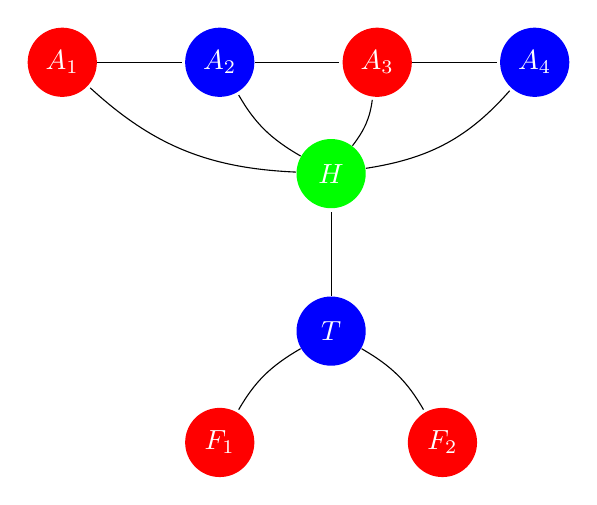
\begin{tikzpicture}[-,>=stealth',shorten >=1pt,auto,node distance=2cm]
	\tikzstyle{every state}=[fill=white,draw=none,text=black]
	
	\node[state,fill=red,text=white] (A1) {$A_1$};
	\node[state,fill=blue,text=white] (A2) [right of =A1] {$A_2$}; 
	\node[state,fill=red,text=white] (A3) [right of =A2] {$A_3$};
	\node[state,fill=blue,text=white] (A4) [right of =A3] {$A_4$};
	
	\node[state,fill=green,text=white] (H) [below right of=A2] {$H$};
	\node[state,fill=blue,text=white] (T) [below of= H ] {$T$};
	\node[state,fill=red,text=white] (F1) [below left of =T] {$F_1$};
	\node[state,fill=red,text=white] (F2) [below right of= T] {$F_2$};
	
	\path [every edge,-] (H) [bend left=20] edge (A1) 
	edge [bend left=15] (A2)
	edge [bend right=15]  (A3)
	edge [bend right=20] (A4)
	(A1) [bend left=0] edge (A2)
	(A2) [bend left=0]edge (A3) 
	(A3) [bend left=0] edge (A4)
	(T) [bend left=0]  edge (H)
	edge [bend right=15](F1)
	edge [bend left=15] (F2);
	\end{tikzpicture}
	
\end{center}
\section{Problem 3}
\begin{itemize}
	\item Representation 1: $x_i \in \{1,2,3,4,5\}, i=1 \dots 25$ denote the position of house (left to right correspond 1 to 5).
	
	\begin{tabular}{c||c|c||c||c||c||c}
		\hline 
		Attribute & Red & White & ... & British & ... & Zebra \\ 
		\hline 
		Belong to & $x_1$ & $x_2$ &  & $x_6$ &  & $x_{25}$ \\ 
		\hline 
	\end{tabular} 
	\item Representation 2: $A_{ij}$ denote the j attribute of house i.
	
	\begin{tabular}{c||ccccc}
		\hline 
		House&$A_1$&$A_2$&$A_3$&$A_4$&$A_5$\\
		\hline \hline
		1   & Water    & Norwegian  & Yellow             & Daunhill                        & Cat \\
		2   & Tea    & Danish  & Blue             & Blend                        & Horse \\
		3 & Milk   & English & Red              & PallMall                     & Bird  \\
		4  & Coffee & German  & Green            & Prince                       & Zebra \\
		5  & Beer   & Swedish & White & BlueMaster  & Dog \\
		\hline
	\end{tabular} 

	I prefer first representation. Because we can easily represent the statement in question with something like $x_i=1$ or $x_i=x_j+1$. And just solve an linear equation system to get the solution.

\end{itemize}

%\begin{thebibliography}{99}
%\bibitem{1} Silver, David, et al. "Mastering the game of Go with deep neural networks and tree search." Nature 529.7587 (2016): 484-489.
%Publishing Company , 1984-1986.
%\bibitem{2} \url{https://www.quora.com/Are-neural-networks-the-future-of-AI}
%\bibitem{3} \url{https://youtu.be/yCALyQRN3hw?list=PLqYmG7hTraZA7v9Hpbps0QNmJC4L1NE3S&t=11434}
%
%\end{thebibliography}	
	
\end{document}
